\begin{figure}[h]
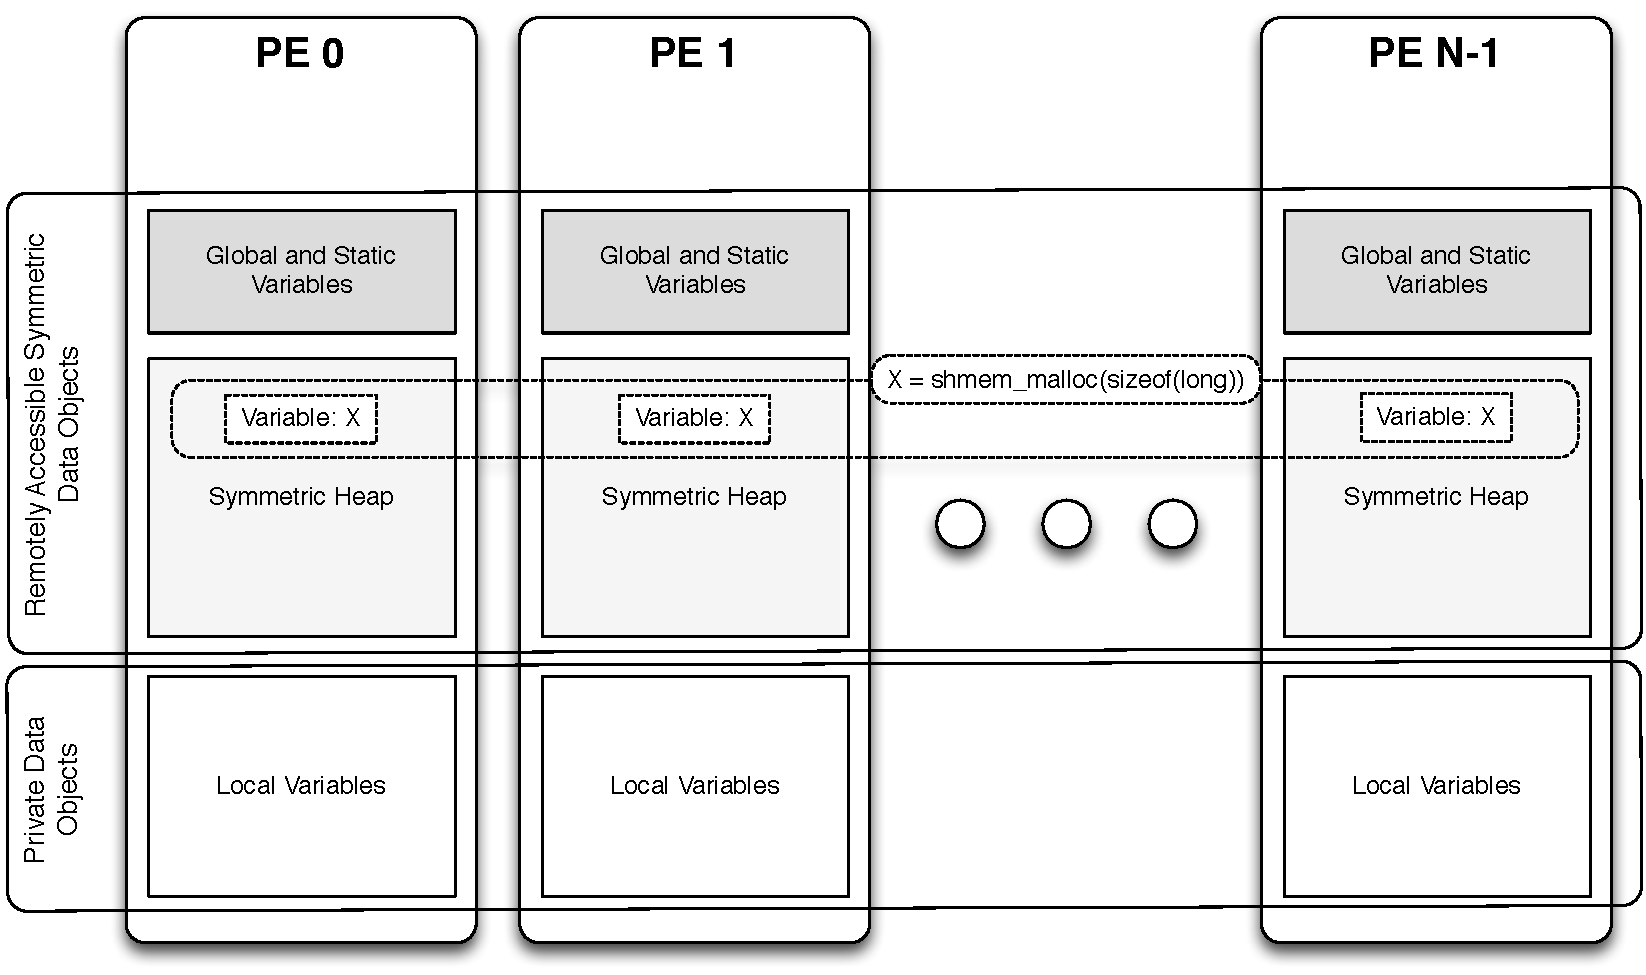
\includegraphics[width=0.95\textwidth]{figures/mem_model}      
\caption{\openshmem Memory Model}
\label{fig:mem_model}                                               
\end{figure}      
%
An \openshmem program consists of data objects that are private to each \ac{PE}
and data  objects that are remotely accessible by all \acp{PE}. Private data
objects are stored in the local memory of each \ac{PE} and can only be accessed
by the \ac{PE} itself; these data objects cannot be accessed by other \acp{PE}
via \openshmem routines. Private data objects follow the memory model of
\Cstd or \Fortran. Remotely accessible objects, however, can be accessed by
remote \acp{PE} using \openshmem routines.  Remotely accessible data objects are
called \emph{Symmetric Data Objects}.  Each symmetric data object has a
corresponding object with the same name, type, and size on all \acp{PE} where that object is
accessible via the \openshmem \ac{API}\footnote{For efficiency reasons,
the same offset (from an arbitrary memory address) for symmetric data
objects might be used on all \acp{PE}. Further discussion about symmetric heap
layout and implementation efficiency can be found in section
\ref{subsec:shfree}}.  (For the definition of what is accessible, see the
descriptions for \FUNC{shmem\_pe\_accessible} and \FUNC{shmem\_addr\_accessible}
in sections \ref{subsec:shmem_pe_accessible} and
\ref{subsec:shmem_addr_accessible}.) Symmetric data objects accessed via typed and
type-generic \openshmem interfaces are required to be naturally aligned based on their type
requirements and underlying architecture.  In \openshmem the following kinds of
data objects are symmetric:
%
\begin{itemize}
\item
  \begin{deprecate}
    \Fortran data objects in common blocks or with the \CTYPE{SAVE} attribute.
    These data objects must not be defined in a dynamic shared object (DSO).
  \end{deprecate}
\item Global and static \Cstd and \Cpp variables. These data objects must
  not  be defined in a DSO.
\item
  \begin{deprecate}
    \Fortran arrays allocated with \FUNC{shpalloc}
  \end{deprecate}
\item \Cstd and \Cpp data allocated by \openshmem memory management routines
  (Section~\ref{sec:memory_management})
\end{itemize}       

\openshmem dynamic memory allocation routines (\FUNC{shpalloc} and
\FUNC{shmem\_malloc}) allow collective allocation of \emph{Symmetric Data
Objects} on a special memory region called the \emph{Symmetric Heap}. The
Symmetric Heap is created during the execution of a program at a memory location
determined by the implementation. The Symmetric Heap may reside in different
memory regions on different \acp{PE}. Figure~\ref{fig:mem_model} shows how
\openshmem implements a \ac{PGAS} model using remotely accessible symmetric
objects and private data objects when executing an \openshmem program.
Symmetric data objects are stored on the symmetric heap or in the global/static
memory section of each \ac{PE}. 
